\documentclass[1p]{elsarticle_modified}
%\bibliographystyle{elsarticle-num}

%\usepackage[colorlinks]{hyperref}
%\usepackage{abbrmath_seonhwa} %\Abb, \Ascr, \Acal ,\Abf, \Afrak
\usepackage{amsfonts}
\usepackage{amssymb}
\usepackage{amsmath}
\usepackage{amsthm}
\usepackage{scalefnt}
\usepackage{amsbsy}
\usepackage{kotex}
\usepackage{caption}
\usepackage{subfig}
\usepackage{color}
\usepackage{graphicx}
\usepackage{xcolor} %% white, black, red, green, blue, cyan, magenta, yellow
\usepackage{float}
\usepackage{setspace}
\usepackage{hyperref}

\usepackage{tikz}
\usetikzlibrary{arrows}

\usepackage{multirow}
\usepackage{array} % fixed length table
\usepackage{hhline}

%%%%%%%%%%%%%%%%%%%%%
\makeatletter
\renewcommand*\env@matrix[1][\arraystretch]{%
	\edef\arraystretch{#1}%
	\hskip -\arraycolsep
	\let\@ifnextchar\new@ifnextchar
	\array{*\c@MaxMatrixCols c}}
\makeatother %https://tex.stackexchange.com/questions/14071/how-can-i-increase-the-line-spacing-in-a-matrix
%%%%%%%%%%%%%%%

\usepackage[normalem]{ulem}

\newcommand{\msout}[1]{\ifmmode\text{\sout{\ensuremath{#1}}}\else\sout{#1}\fi}
%SOURCE: \msout is \stkout macro in https://tex.stackexchange.com/questions/20609/strikeout-in-math-mode

\newcommand{\cancel}[1]{
	\ifmmode
	{\color{red}\msout{#1}}
	\else
	{\color{red}\sout{#1}}
	\fi
}

\newcommand{\add}[1]{
	{\color{blue}\uwave{#1}}
}

\newcommand{\replace}[2]{
	\ifmmode
	{\color{red}\msout{#1}}{\color{blue}\uwave{#2}}
	\else
	{\color{red}\sout{#1}}{\color{blue}\uwave{#2}}
	\fi
}

\newcommand{\Sol}{\mathcal{S}} %segment
\newcommand{\D}{D} %diagram
\newcommand{\A}{\mathcal{A}} %arc


%%%%%%%%%%%%%%%%%%%%%%%%%%%%%5 test

\def\sl{\operatorname{\textup{SL}}(2,\Cbb)}
\def\psl{\operatorname{\textup{PSL}}(2,\Cbb)}
\def\quan{\mkern 1mu \triangleright \mkern 1mu}

\theoremstyle{definition}
\newtheorem{thm}{Theorem}[section]
\newtheorem{prop}[thm]{Proposition}
\newtheorem{lem}[thm]{Lemma}
\newtheorem{ques}[thm]{Question}
\newtheorem{cor}[thm]{Corollary}
\newtheorem{defn}[thm]{Definition}
\newtheorem{exam}[thm]{Example}
\newtheorem{rmk}[thm]{Remark}
\newtheorem{alg}[thm]{Algorithm}

\newcommand{\I}{\sqrt{-1}}
\begin{document}

%\begin{frontmatter}
%
%\title{Boundary parabolic representations of knots up to 8 crossings}
%
%%% Group authors per affiliation:
%\author{Yunhi Cho} 
%\address{Department of Mathematics, University of Seoul, Seoul, Korea}
%\ead{yhcho@uos.ac.kr}
%
%
%\author{Seonhwa Kim} %\fnref{s_kim}}
%\address{Center for Geometry and Physics, Institute for Basic Science, Pohang, 37673, Korea}
%\ead{ryeona17@ibs.re.kr}
%
%\author{Hyuk Kim}
%\address{Department of Mathematical Sciences, Seoul National University, Seoul 08826, Korea}
%\ead{hyukkim@snu.ac.kr}
%
%\author{Seokbeom Yoon}
%\address{Department of Mathematical Sciences, Seoul National University, Seoul, 08826,  Korea}
%\ead{sbyoon15@snu.ac.kr}
%
%\begin{abstract}
%We find all boundary parabolic representation of knots up to 8 crossings.
%
%\end{abstract}
%\begin{keyword}
%    \MSC[2010] 57M25 
%\end{keyword}
%
%\end{frontmatter}

%\linenumbers
%\tableofcontents
%
\newcommand\colored[1]{\textcolor{white}{\rule[-0.35ex]{0.8em}{1.4ex}}\kern-0.8em\color{red} #1}%
%\newcommand\colored[1]{\textcolor{white}{ #1}\kern-2.17ex	\textcolor{white}{ #1}\kern-1.81ex	\textcolor{white}{ #1}\kern-2.15ex\color{red}#1	}

{\Large $\underline{12n_{0004}~(K12n_{0004})}$}

\setlength{\tabcolsep}{10pt}
\renewcommand{\arraystretch}{1.6}
\vspace{1cm}\begin{tabular}{m{100pt}>{\centering\arraybackslash}m{274pt}}
\multirow{5}{120pt}{
	\centering
	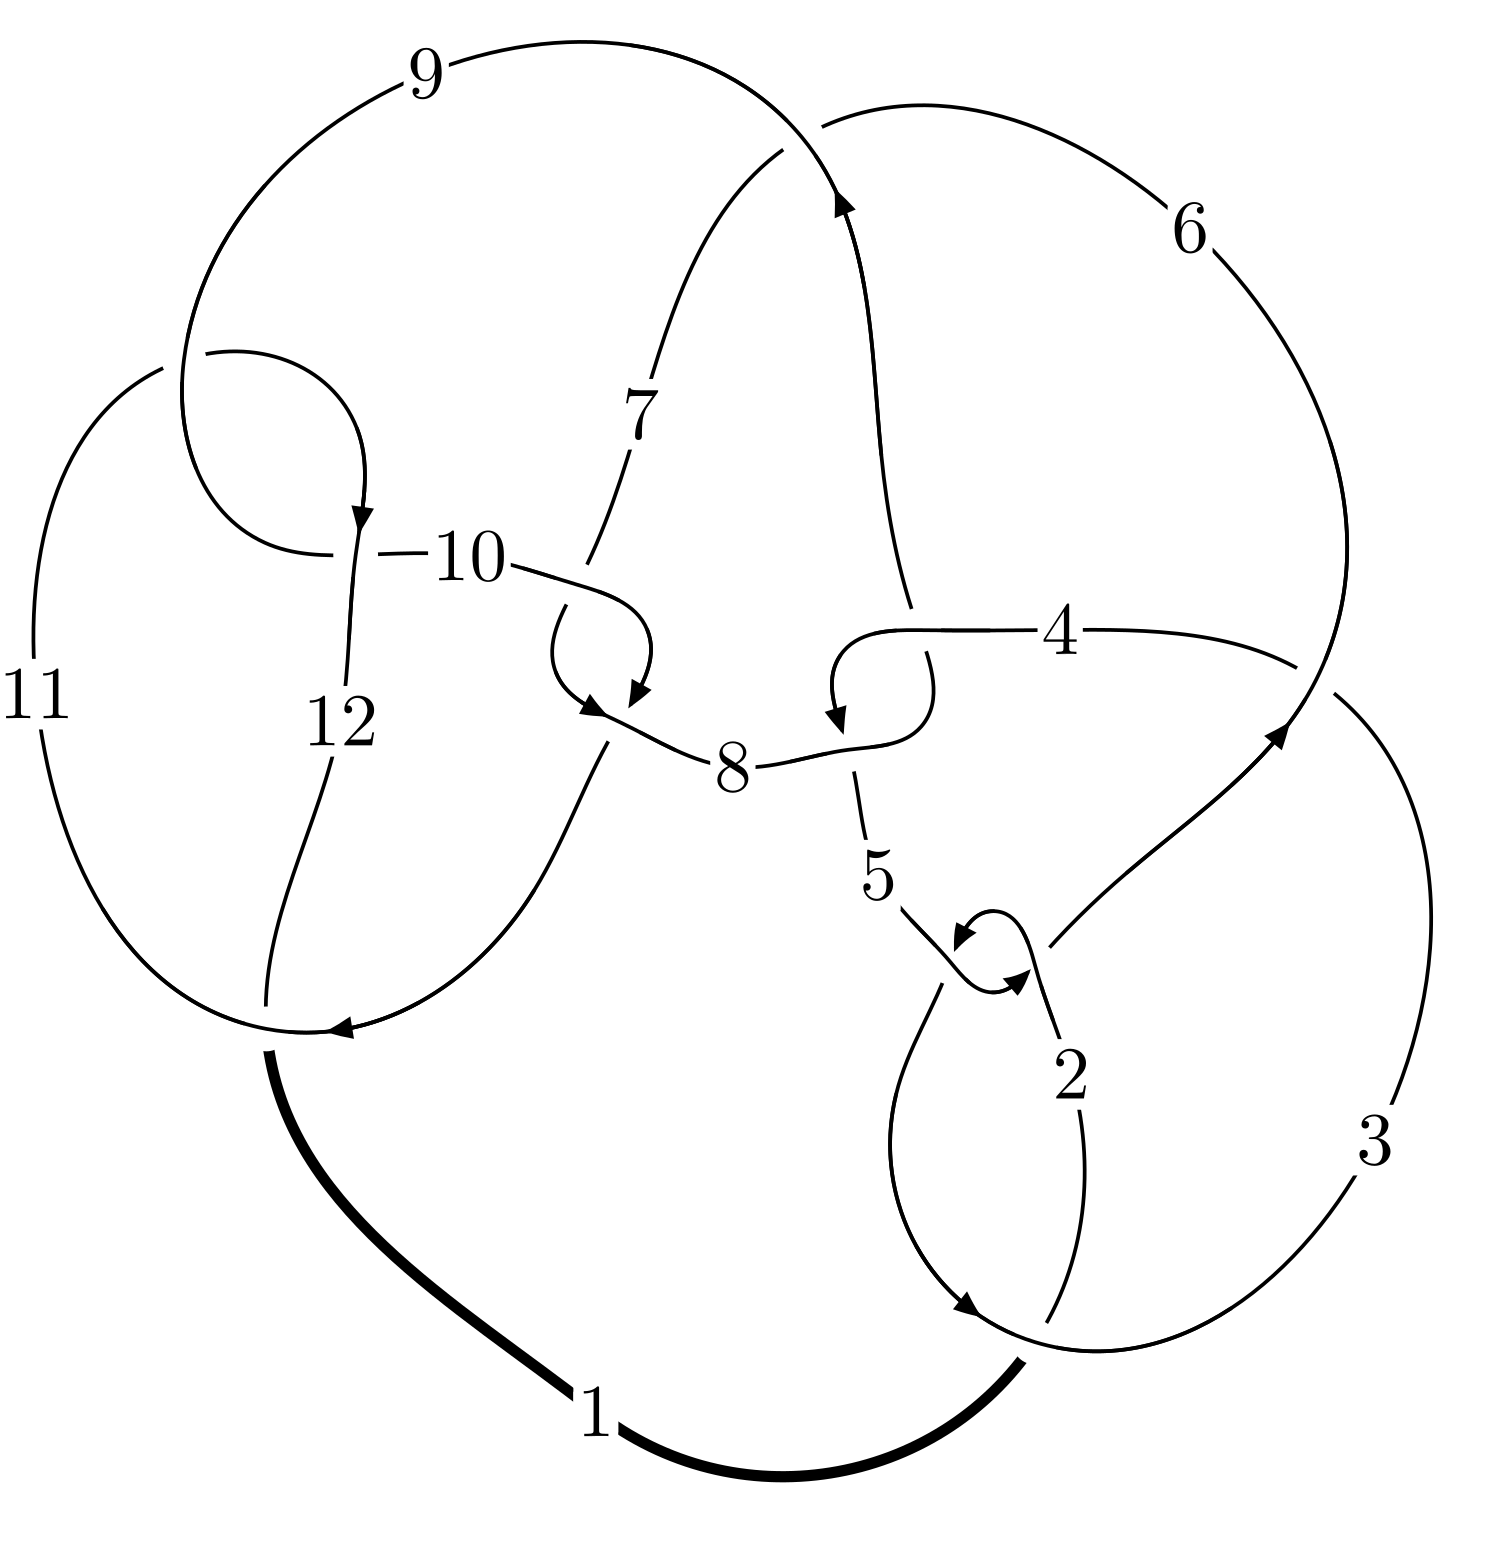
\includegraphics[width=112pt]{../../../GIT/diagram.site/Diagrams/png/2093_12n_0004.png}\\
\ \ \ A knot diagram\footnotemark}&
\allowdisplaybreaks
\textbf{Linearized knot diagam} \\
\cline{2-2}
 &
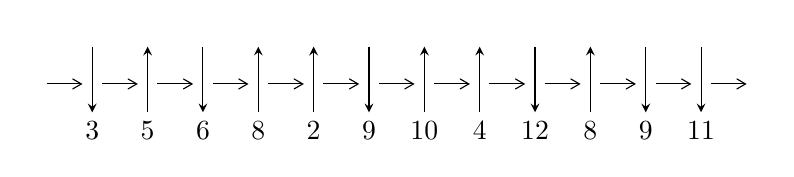
\begin{tikzpicture}[x=20pt, y=17pt]
	% nodes
	\node (C0) at (0, 0) {};
	\node (C1) at (1, 0) {};
	\node (C1U) at (1, +1) {};
	\node (C1D) at (1, -1) {3};

	\node (C2) at (2, 0) {};
	\node (C2U) at (2, +1) {};
	\node (C2D) at (2, -1) {5};

	\node (C3) at (3, 0) {};
	\node (C3U) at (3, +1) {};
	\node (C3D) at (3, -1) {6};

	\node (C4) at (4, 0) {};
	\node (C4U) at (4, +1) {};
	\node (C4D) at (4, -1) {8};

	\node (C5) at (5, 0) {};
	\node (C5U) at (5, +1) {};
	\node (C5D) at (5, -1) {2};

	\node (C6) at (6, 0) {};
	\node (C6U) at (6, +1) {};
	\node (C6D) at (6, -1) {9};

	\node (C7) at (7, 0) {};
	\node (C7U) at (7, +1) {};
	\node (C7D) at (7, -1) {10};

	\node (C8) at (8, 0) {};
	\node (C8U) at (8, +1) {};
	\node (C8D) at (8, -1) {4};

	\node (C9) at (9, 0) {};
	\node (C9U) at (9, +1) {};
	\node (C9D) at (9, -1) {12};

	\node (C10) at (10, 0) {};
	\node (C10U) at (10, +1) {};
	\node (C10D) at (10, -1) {8};

	\node (C11) at (11, 0) {};
	\node (C11U) at (11, +1) {};
	\node (C11D) at (11, -1) {9};

	\node (C12) at (12, 0) {};
	\node (C12U) at (12, +1) {};
	\node (C12D) at (12, -1) {11};
	\node (C13) at (13, 0) {};

	% arrows
	\draw[->,>={angle 60}]
	(C0) edge (C1) (C1) edge (C2) (C2) edge (C3) (C3) edge (C4) (C4) edge (C5) (C5) edge (C6) (C6) edge (C7) (C7) edge (C8) (C8) edge (C9) (C9) edge (C10) (C10) edge (C11) (C11) edge (C12) (C12) edge (C13) ;	\draw[->,>=stealth]
	(C1U) edge (C1D) (C2D) edge (C2U) (C3U) edge (C3D) (C4D) edge (C4U) (C5D) edge (C5U) (C6U) edge (C6D) (C7D) edge (C7U) (C8D) edge (C8U) (C9U) edge (C9D) (C10D) edge (C10U) (C11U) edge (C11D) (C12U) edge (C12D) ;
	\end{tikzpicture} \\
\hhline{~~} \\& 
\textbf{Solving Sequence} \\ \cline{2-2} 
 &
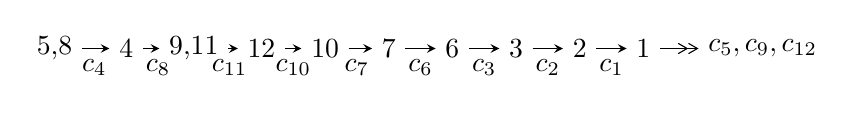
\begin{tikzpicture}[x=23pt, y=7pt]
	% node
	\node (A0) at (-1/8, 0) {5,8};
	\node (A1) at (1, 0) {4};
	\node (A2) at (33/16, 0) {9,11};
	\node (A3) at (25/8, 0) {12};
	\node (A4) at (33/8, 0) {10};
	\node (A5) at (41/8, 0) {7};
	\node (A6) at (49/8, 0) {6};
	\node (A7) at (57/8, 0) {3};
	\node (A8) at (65/8, 0) {2};
	\node (A9) at (73/8, 0) {1};
	\node (C1) at (1/2, -1) {$c_{4}$};
	\node (C2) at (3/2, -1) {$c_{8}$};
	\node (C3) at (21/8, -1) {$c_{11}$};
	\node (C4) at (29/8, -1) {$c_{10}$};
	\node (C5) at (37/8, -1) {$c_{7}$};
	\node (C6) at (45/8, -1) {$c_{6}$};
	\node (C7) at (53/8, -1) {$c_{3}$};
	\node (C8) at (61/8, -1) {$c_{2}$};
	\node (C9) at (69/8, -1) {$c_{1}$};
	\node (A10) at (11, 0) {$c_{5},c_{9},c_{12}$};

	% edge
	\draw[->,>=stealth]	
	(A0) edge (A1) (A1) edge (A2) (A2) edge (A3) (A3) edge (A4) (A4) edge (A5) (A5) edge (A6) (A6) edge (A7) (A7) edge (A8) (A8) edge (A9) ;
	\draw[->>,>={angle 60}]	
	(A9) edge (A10);
\end{tikzpicture} \\ 

\end{tabular} \\

\footnotetext{
The image of knot diagram is generated by the software ``\textbf{Draw programme}" developed by Andrew Bartholomew(\url{http://www.layer8.co.uk/maths/draw/index.htm\#Running-draw}), where we modified some parts for our purpose(\url{https://github.com/CATsTAILs/LinksPainter}).
}\phantom \\ \newline 
\centering \textbf{Ideals for irreducible components\footnotemark of $X_{\text{par}}$} 
 
\begin{align*}
I^u_{1}&=\langle 
2.68313\times10^{45} u^{49}+5.65169\times10^{45} u^{48}+\cdots+2.22303\times10^{45} b+2.08265\times10^{45},\\
\phantom{I^u_{1}}&\phantom{= \langle  }5.37170\times10^{43} u^{49}+1.30102\times10^{44} u^{48}+\cdots+2.22303\times10^{45} a-4.96236\times10^{44},\;u^{50}+2 u^{49}+\cdots+u+1\rangle \\
I^u_{2}&=\langle 
u^3+b+u+1,\;a,\;u^4+u^2+u+1\rangle \\
I^u_{3}&=\langle 
u^5- u^4+2 u^3-2 u^2+b+2 u-2,\;a,\;u^6- u^5+2 u^4-2 u^3+2 u^2-2 u+1\rangle \\
\\
\end{align*}
\raggedright * 3 irreducible components of $\dim_{\mathbb{C}}=0$, with total 60 representations.\\
\footnotetext{All coefficients of polynomials are rational numbers. But the coefficients are sometimes approximated in decimal forms when there is not enough margin.}
\newpage
\renewcommand{\arraystretch}{1}
\centering \section*{I. $I^u_{1}= \langle 2.68\times10^{45} u^{49}+5.65\times10^{45} u^{48}+\cdots+2.22\times10^{45} b+2.08\times10^{45},\;5.37\times10^{43} u^{49}+1.30\times10^{44} u^{48}+\cdots+2.22\times10^{45} a-4.96\times10^{44},\;u^{50}+2 u^{49}+\cdots+u+1 \rangle$}
\flushleft \textbf{(i) Arc colorings}\\
\begin{tabular}{m{7pt} m{180pt} m{7pt} m{180pt} }
\flushright $a_{5}=$&$\begin{pmatrix}1\\0\end{pmatrix}$ \\
\flushright $a_{8}=$&$\begin{pmatrix}0\\u\end{pmatrix}$ \\
\flushright $a_{4}=$&$\begin{pmatrix}1\\u^2\end{pmatrix}$ \\
\flushright $a_{9}=$&$\begin{pmatrix}u\\u^3+u\end{pmatrix}$ \\
\flushright $a_{11}=$&$\begin{pmatrix}-0.0241638 u^{49}-0.0585243 u^{48}+\cdots+2.46234 u+0.223225\\-1.20697 u^{49}-2.54233 u^{48}+\cdots-1.10388 u-0.936850\end{pmatrix}$ \\
\flushright $a_{12}=$&$\begin{pmatrix}u\\-1.23912 u^{49}-2.70146 u^{48}+\cdots-2.60058 u-1.17027\end{pmatrix}$ \\
\flushright $a_{10}=$&$\begin{pmatrix}-0.0241638 u^{49}-0.0585243 u^{48}+\cdots+2.46234 u+0.223225\\-1.15066 u^{49}-2.32468 u^{48}+\cdots-1.06952 u-0.926653\end{pmatrix}$ \\
\flushright $a_{7}=$&$\begin{pmatrix}-0.172888 u^{49}-0.633762 u^{48}+\cdots-0.157137 u-0.0708064\\-0.00568877 u^{49}-0.0730463 u^{48}+\cdots-0.998737 u+0.163739\end{pmatrix}$ \\
\flushright $a_{6}=$&$\begin{pmatrix}-0.296253 u^{49}-0.972434 u^{48}+\cdots-0.415283 u-0.214269\\-0.0837652 u^{49}-0.360352 u^{48}+\cdots-1.04157 u+0.112220\end{pmatrix}$ \\
\flushright $a_{3}=$&$\begin{pmatrix}-0.0373866 u^{49}+0.100580 u^{48}+\cdots-0.326440 u+1.04404\\0.373816 u^{49}+0.661193 u^{48}+\cdots-0.0581820 u-0.269424\end{pmatrix}$ \\
\flushright $a_{2}=$&$\begin{pmatrix}-0.411203 u^{49}-0.560613 u^{48}+\cdots-0.268258 u+1.31346\\0.373816 u^{49}+0.661193 u^{48}+\cdots-0.0581820 u-0.269424\end{pmatrix}$ \\
\flushright $a_{1}=$&$\begin{pmatrix}-0.114683 u^{49}-0.372829 u^{48}+\cdots+1.30247 u+0.0534395\\0.181570 u^{49}+0.599605 u^{48}+\cdots+1.71776 u+0.267709\end{pmatrix}$\\&\end{tabular}
\flushleft \textbf{(ii) Obstruction class $= -1$}\\~\\
\flushleft \textbf{(iii) Cusp Shapes $= 4.70229 u^{49}+5.71053 u^{48}+\cdots-8.33362 u-6.55580$}\\~\\
\newpage\renewcommand{\arraystretch}{1}
\flushleft \textbf{(iv) u-Polynomials at the component}\newline \\
\begin{tabular}{m{50pt}|m{274pt}}
Crossings & \hspace{64pt}u-Polynomials at each crossing \\
\hline $$\begin{aligned}c_{1}\end{aligned}$$&$\begin{aligned}
&u^{50}+22 u^{49}+\cdots+5 u+1
\end{aligned}$\\
\hline $$\begin{aligned}c_{2},c_{5}\end{aligned}$$&$\begin{aligned}
&u^{50}+2 u^{49}+\cdots+5 u+1
\end{aligned}$\\
\hline $$\begin{aligned}c_{3}\end{aligned}$$&$\begin{aligned}
&u^{50}-2 u^{49}+\cdots-48 u+36
\end{aligned}$\\
\hline $$\begin{aligned}c_{4},c_{8}\end{aligned}$$&$\begin{aligned}
&u^{50}-2 u^{49}+\cdots- u+1
\end{aligned}$\\
\hline $$\begin{aligned}c_{6}\end{aligned}$$&$\begin{aligned}
&u^{50}-10 u^{49}+\cdots-6028015 u+3579401
\end{aligned}$\\
\hline $$\begin{aligned}c_{7},c_{10}\end{aligned}$$&$\begin{aligned}
&u^{50}+5 u^{49}+\cdots+5120 u+1024
\end{aligned}$\\
\hline $$\begin{aligned}c_{9},c_{11}\end{aligned}$$&$\begin{aligned}
&u^{50}-11 u^{49}+\cdots-10 u+1
\end{aligned}$\\
\hline $$\begin{aligned}c_{12}\end{aligned}$$&$\begin{aligned}
&u^{50}+9 u^{49}+\cdots-10 u+1
\end{aligned}$\\
\hline
\end{tabular}\\~\\
\newpage\renewcommand{\arraystretch}{1}
\flushleft \textbf{(v) Riley Polynomials at the component}\newline \\
\begin{tabular}{m{50pt}|m{274pt}}
Crossings & \hspace{64pt}Riley Polynomials at each crossing \\
\hline $$\begin{aligned}c_{1}\end{aligned}$$&$\begin{aligned}
&y^{50}+14 y^{49}+\cdots+105 y+1
\end{aligned}$\\
\hline $$\begin{aligned}c_{2},c_{5}\end{aligned}$$&$\begin{aligned}
&y^{50}+22 y^{49}+\cdots+5 y+1
\end{aligned}$\\
\hline $$\begin{aligned}c_{3}\end{aligned}$$&$\begin{aligned}
&y^{50}+6 y^{49}+\cdots+28872 y+1296
\end{aligned}$\\
\hline $$\begin{aligned}c_{4},c_{8}\end{aligned}$$&$\begin{aligned}
&y^{50}+10 y^{49}+\cdots+5 y+1
\end{aligned}$\\
\hline $$\begin{aligned}c_{6}\end{aligned}$$&$\begin{aligned}
&y^{50}+74 y^{49}+\cdots+905556314476485 y+12812111518801
\end{aligned}$\\
\hline $$\begin{aligned}c_{7},c_{10}\end{aligned}$$&$\begin{aligned}
&y^{50}-63 y^{49}+\cdots-14155776 y+1048576
\end{aligned}$\\
\hline $$\begin{aligned}c_{9},c_{11}\end{aligned}$$&$\begin{aligned}
&y^{50}-9 y^{49}+\cdots+10 y+1
\end{aligned}$\\
\hline $$\begin{aligned}c_{12}\end{aligned}$$&$\begin{aligned}
&y^{50}+75 y^{49}+\cdots+10 y+1
\end{aligned}$\\
\hline
\end{tabular}\\~\\
\newpage\flushleft \textbf{(vi) Complex Volumes and Cusp Shapes}
$$\begin{array}{c|c|c}  
\text{Solutions to }I^u_{1}& \I (\text{vol} + \sqrt{-1}CS) & \text{Cusp shape}\\
 \hline 
\begin{aligned}
u &= \phantom{-}0.585003 + 0.735265 I \\
a &= \phantom{-}1.57008 + 0.40175 I \\
b &= \phantom{-}0.294139 + 0.670355 I\end{aligned}
 & \phantom{-}0.18981 + 6.85618 I & -0.26689 - 9.43060 I \\ \hline\begin{aligned}
u &= \phantom{-}0.585003 - 0.735265 I \\
a &= \phantom{-}1.57008 - 0.40175 I \\
b &= \phantom{-}0.294139 - 0.670355 I\end{aligned}
 & \phantom{-}0.18981 - 6.85618 I & -0.26689 + 9.43060 I \\ \hline\begin{aligned}
u &= \phantom{-}0.892429 + 0.266725 I \\
a &= \phantom{-}0.668641 - 0.033988 I \\
b &= \phantom{-}0.763934 + 0.111453 I\end{aligned}
 & -0.49506 - 3.19030 I & \phantom{-}2.46244 + 4.05593 I \\ \hline\begin{aligned}
u &= \phantom{-}0.892429 - 0.266725 I \\
a &= \phantom{-}0.668641 + 0.033988 I \\
b &= \phantom{-}0.763934 - 0.111453 I\end{aligned}
 & -0.49506 + 3.19030 I & \phantom{-}2.46244 - 4.05593 I \\ \hline\begin{aligned}
u &= -0.627517 + 0.673413 I \\
a &= -1.357940 + 0.261790 I \\
b &= -0.510233 + 0.568117 I\end{aligned}
 & \phantom{-}1.65860 - 2.16501 I & \phantom{-}3.61128 + 3.98050 I \\ \hline\begin{aligned}
u &= -0.627517 - 0.673413 I \\
a &= -1.357940 - 0.261790 I \\
b &= -0.510233 - 0.568117 I\end{aligned}
 & \phantom{-}1.65860 + 2.16501 I & \phantom{-}3.61128 - 3.98050 I \\ \hline\begin{aligned}
u &= -0.412013 + 0.747742 I \\
a &= -0.058407 + 0.811246 I \\
b &= \phantom{-}0.131377 + 0.894939 I\end{aligned}
 & \phantom{-}1.19055 - 1.89480 I & \phantom{-}3.58493 + 4.65187 I \\ \hline\begin{aligned}
u &= -0.412013 - 0.747742 I \\
a &= -0.058407 - 0.811246 I \\
b &= \phantom{-}0.131377 - 0.894939 I\end{aligned}
 & \phantom{-}1.19055 + 1.89480 I & \phantom{-}3.58493 - 4.65187 I \\ \hline\begin{aligned}
u &= -0.713195 + 0.463752 I \\
a &= -0.882675 + 0.101195 I \\
b &= -0.711974 + 0.297517 I\end{aligned}
 & \phantom{-}1.34929 - 0.89664 I & \phantom{-}5.51965 + 2.35436 I \\ \hline\begin{aligned}
u &= -0.713195 - 0.463752 I \\
a &= -0.882675 - 0.101195 I \\
b &= -0.711974 - 0.297517 I\end{aligned}
 & \phantom{-}1.34929 + 0.89664 I & \phantom{-}5.51965 - 2.35436 I\\
 \hline 
 \end{array}$$\newpage$$\begin{array}{c|c|c}  
\text{Solutions to }I^u_{1}& \I (\text{vol} + \sqrt{-1}CS) & \text{Cusp shape}\\
 \hline 
\begin{aligned}
u &= -0.442833 + 1.118810 I \\
a &= \phantom{-}0.228660 + 0.614406 I \\
b &= \phantom{-}0.496365 + 0.310678 I\end{aligned}
 & -0.96543 - 3.58766 I & \phantom{-}2.90819 + 4.89226 I \\ \hline\begin{aligned}
u &= -0.442833 - 1.118810 I \\
a &= \phantom{-}0.228660 - 0.614406 I \\
b &= \phantom{-}0.496365 - 0.310678 I\end{aligned}
 & -0.96543 + 3.58766 I & \phantom{-}2.90819 - 4.89226 I \\ \hline\begin{aligned}
u &= \phantom{-}0.415615 + 0.648154 I \\
a &= \phantom{-}1.13644 + 0.88310 I \\
b &= \phantom{-}0.232356 + 0.006577 I\end{aligned}
 & -2.15443 + 1.20962 I & -5.26784 - 4.21990 I \\ \hline\begin{aligned}
u &= \phantom{-}0.415615 - 0.648154 I \\
a &= \phantom{-}1.13644 - 0.88310 I \\
b &= \phantom{-}0.232356 - 0.006577 I\end{aligned}
 & -2.15443 - 1.20962 I & -5.26784 + 4.21990 I \\ \hline\begin{aligned}
u &= -0.239224 + 0.729553 I \\
a &= -0.92587 + 1.52769 I \\
b &= \phantom{-}0.184105 - 0.655650 I\end{aligned}
 & -3.56813 - 4.51753 I & -7.12654 + 7.85182 I \\ \hline\begin{aligned}
u &= -0.239224 - 0.729553 I \\
a &= -0.92587 - 1.52769 I \\
b &= \phantom{-}0.184105 + 0.655650 I\end{aligned}
 & -3.56813 + 4.51753 I & -7.12654 - 7.85182 I \\ \hline\begin{aligned}
u &= \phantom{-}0.474690 + 0.586628 I \\
a &= \phantom{-}0.317436 + 0.867818 I \\
b &= \phantom{-}0.336934 + 1.108570 I\end{aligned}
 & \phantom{-}0.36504 - 2.86959 I & \phantom{-}1.52034 + 1.42682 I \\ \hline\begin{aligned}
u &= \phantom{-}0.474690 - 0.586628 I \\
a &= \phantom{-}0.317436 - 0.867818 I \\
b &= \phantom{-}0.336934 - 1.108570 I\end{aligned}
 & \phantom{-}0.36504 + 2.86959 I & \phantom{-}1.52034 - 1.42682 I \\ \hline\begin{aligned}
u &= \phantom{-}0.276652 + 1.215690 I \\
a &= -0.130051 + 0.523865 I \\
b &= -0.256894 + 0.216714 I\end{aligned}
 & -5.21381 + 0.38052 I & \phantom{-0.000000 } 0 \\ \hline\begin{aligned}
u &= \phantom{-}0.276652 - 1.215690 I \\
a &= -0.130051 - 0.523865 I \\
b &= -0.256894 - 0.216714 I\end{aligned}
 & -5.21381 - 0.38052 I & \phantom{-0.000000 } 0\\
 \hline 
 \end{array}$$\newpage$$\begin{array}{c|c|c}  
\text{Solutions to }I^u_{1}& \I (\text{vol} + \sqrt{-1}CS) & \text{Cusp shape}\\
 \hline 
\begin{aligned}
u &= -0.932827 + 0.874426 I \\
a &= -1.22918 - 1.02414 I \\
b &= -1.88245 + 0.61714 I\end{aligned}
 & \phantom{-}8.53540 - 6.83590 I & \phantom{-0.000000 } 0 \\ \hline\begin{aligned}
u &= -0.932827 - 0.874426 I \\
a &= -1.22918 + 1.02414 I \\
b &= -1.88245 - 0.61714 I\end{aligned}
 & \phantom{-}8.53540 + 6.83590 I & \phantom{-0.000000 } 0 \\ \hline\begin{aligned}
u &= -0.084592 + 0.713079 I \\
a &= -0.33510 + 1.70480 I \\
b &= \phantom{-}0.060912 - 1.093010 I\end{aligned}
 & -4.25283 + 1.34403 I & -9.08170 - 1.74638 I \\ \hline\begin{aligned}
u &= -0.084592 - 0.713079 I \\
a &= -0.33510 - 1.70480 I \\
b &= \phantom{-}0.060912 + 1.093010 I\end{aligned}
 & -4.25283 - 1.34403 I & -9.08170 + 1.74638 I \\ \hline\begin{aligned}
u &= -0.986608 + 0.831816 I \\
a &= -0.974415 - 0.890813 I \\
b &= -1.69006 + 0.29018 I\end{aligned}
 & \phantom{-}4.09805 + 0.13420 I & \phantom{-0.000000 } 0 \\ \hline\begin{aligned}
u &= -0.986608 - 0.831816 I \\
a &= -0.974415 + 0.890813 I \\
b &= -1.69006 - 0.29018 I\end{aligned}
 & \phantom{-}4.09805 - 0.13420 I & \phantom{-0.000000 } 0 \\ \hline\begin{aligned}
u &= \phantom{-}0.953965 + 0.875078 I \\
a &= \phantom{-}1.13306 - 1.04945 I \\
b &= \phantom{-}1.91375 + 0.48552 I\end{aligned}
 & \phantom{-}10.16820 + 1.33885 I & \phantom{-0.000000 } 0 \\ \hline\begin{aligned}
u &= \phantom{-}0.953965 - 0.875078 I \\
a &= \phantom{-}1.13306 + 1.04945 I \\
b &= \phantom{-}1.91375 - 0.48552 I\end{aligned}
 & \phantom{-}10.16820 - 1.33885 I & \phantom{-0.000000 } 0 \\ \hline\begin{aligned}
u &= \phantom{-}0.503491 + 1.215080 I \\
a &= -0.292017 + 0.535955 I \\
b &= -0.543268 + 0.125989 I\end{aligned}
 & -3.59441 + 8.42989 I & \phantom{-0.000000 } 0 \\ \hline\begin{aligned}
u &= \phantom{-}0.503491 - 1.215080 I \\
a &= -0.292017 - 0.535955 I \\
b &= -0.543268 - 0.125989 I\end{aligned}
 & -3.59441 - 8.42989 I & \phantom{-0.000000 } 0\\
 \hline 
 \end{array}$$\newpage$$\begin{array}{c|c|c}  
\text{Solutions to }I^u_{1}& \I (\text{vol} + \sqrt{-1}CS) & \text{Cusp shape}\\
 \hline 
\begin{aligned}
u &= -0.864809 + 0.998500 I \\
a &= \phantom{-}1.021580 + 0.934002 I \\
b &= \phantom{-}2.26238 + 0.01234 I\end{aligned}
 & \phantom{-}8.12452 + 0.19479 I & \phantom{-0.000000 } 0 \\ \hline\begin{aligned}
u &= -0.864809 - 0.998500 I \\
a &= \phantom{-}1.021580 - 0.934002 I \\
b &= \phantom{-}2.26238 - 0.01234 I\end{aligned}
 & \phantom{-}8.12452 - 0.19479 I & \phantom{-0.000000 } 0 \\ \hline\begin{aligned}
u &= \phantom{-}1.004750 + 0.876459 I \\
a &= \phantom{-}0.905947 - 1.070140 I \\
b &= \phantom{-}1.91696 + 0.17358 I\end{aligned}
 & \phantom{-}9.78917 - 2.20715 I & \phantom{-0.000000 } 0 \\ \hline\begin{aligned}
u &= \phantom{-}1.004750 - 0.876459 I \\
a &= \phantom{-}0.905947 + 1.070140 I \\
b &= \phantom{-}1.91696 - 0.17358 I\end{aligned}
 & \phantom{-}9.78917 + 2.20715 I & \phantom{-0.000000 } 0 \\ \hline\begin{aligned}
u &= \phantom{-}0.879539 + 1.011550 I \\
a &= -1.081270 + 0.875542 I \\
b &= -2.29261 - 0.17584 I\end{aligned}
 & \phantom{-}9.71806 + 5.41424 I & \phantom{-0.000000 } 0 \\ \hline\begin{aligned}
u &= \phantom{-}0.879539 - 1.011550 I \\
a &= -1.081270 - 0.875542 I \\
b &= -2.29261 + 0.17584 I\end{aligned}
 & \phantom{-}9.71806 - 5.41424 I & \phantom{-0.000000 } 0 \\ \hline\begin{aligned}
u &= -1.024250 + 0.878258 I \\
a &= -0.822290 - 1.069240 I \\
b &= -1.90015 + 0.05959 I\end{aligned}
 & \phantom{-}7.85339 + 7.67379 I & \phantom{-0.000000 } 0 \\ \hline\begin{aligned}
u &= -1.024250 - 0.878258 I \\
a &= -0.822290 + 1.069240 I \\
b &= -1.90015 - 0.05959 I\end{aligned}
 & \phantom{-}7.85339 - 7.67379 I & \phantom{-0.000000 } 0 \\ \hline\begin{aligned}
u &= -0.877514 + 1.052570 I \\
a &= \phantom{-}1.041610 + 0.710120 I \\
b &= \phantom{-}1.99699 - 0.41591 I\end{aligned}
 & \phantom{-}3.38860 - 6.97331 I & \phantom{-0.000000 } 0 \\ \hline\begin{aligned}
u &= -0.877514 - 1.052570 I \\
a &= \phantom{-}1.041610 - 0.710120 I \\
b &= \phantom{-}1.99699 + 0.41591 I\end{aligned}
 & \phantom{-}3.38860 + 6.97331 I & \phantom{-0.000000 } 0\\
 \hline 
 \end{array}$$\newpage$$\begin{array}{c|c|c}  
\text{Solutions to }I^u_{1}& \I (\text{vol} + \sqrt{-1}CS) & \text{Cusp shape}\\
 \hline 
\begin{aligned}
u &= \phantom{-}0.241768 + 0.574851 I \\
a &= \phantom{-}0.656765 + 1.098310 I \\
b &= \phantom{-}0.388520 - 0.721943 I\end{aligned}
 & -1.91283 + 0.92101 I & -3.25247 - 0.86020 I \\ \hline\begin{aligned}
u &= \phantom{-}0.241768 - 0.574851 I \\
a &= \phantom{-}0.656765 - 1.098310 I \\
b &= \phantom{-}0.388520 + 0.721943 I\end{aligned}
 & -1.91283 - 0.92101 I & -3.25247 + 0.86020 I \\ \hline\begin{aligned}
u &= \phantom{-}0.907639 + 1.041190 I \\
a &= -1.179790 + 0.720010 I \\
b &= -2.25110 - 0.59042 I\end{aligned}
 & \phantom{-}9.24238 + 9.20482 I & \phantom{-0.000000 } 0 \\ \hline\begin{aligned}
u &= \phantom{-}0.907639 - 1.041190 I \\
a &= -1.179790 - 0.720010 I \\
b &= -2.25110 + 0.59042 I\end{aligned}
 & \phantom{-}9.24238 - 9.20482 I & \phantom{-0.000000 } 0 \\ \hline\begin{aligned}
u &= -0.916608 + 1.051050 I \\
a &= \phantom{-}1.204760 + 0.661896 I \\
b &= \phantom{-}2.21127 - 0.72670 I\end{aligned}
 & \phantom{-}7.2749 - 14.7585 I & \phantom{-0.000000 } 0 \\ \hline\begin{aligned}
u &= -0.916608 - 1.051050 I \\
a &= \phantom{-}1.204760 - 0.661896 I \\
b &= \phantom{-}2.21127 + 0.72670 I\end{aligned}
 & \phantom{-}7.2749 + 14.7585 I & \phantom{-0.000000 } 0 \\ \hline\begin{aligned}
u &= \phantom{-}0.418143 + 0.325356 I \\
a &= \phantom{-}0.746640 + 0.640935 I \\
b &= \phantom{-}2.00114 + 0.03022 I\end{aligned}
 & -1.36557 + 1.46875 I & -6.84223 - 10.34978 I \\ \hline\begin{aligned}
u &= \phantom{-}0.418143 - 0.325356 I \\
a &= \phantom{-}0.746640 - 0.640935 I \\
b &= \phantom{-}2.00114 - 0.03022 I\end{aligned}
 & -1.36557 - 1.46875 I & -6.84223 + 10.34978 I \\ \hline\begin{aligned}
u &= -0.431697 + 0.145919 I \\
a &= -0.862616 + 0.330550 I \\
b &= -3.15240 - 0.05844 I\end{aligned}
 & -1.85076 + 2.37111 I & \phantom{-}9.8016 + 19.1551 I \\ \hline\begin{aligned}
u &= -0.431697 - 0.145919 I \\
a &= -0.862616 - 0.330550 I \\
b &= -3.15240 + 0.05844 I\end{aligned}
 & -1.85076 - 2.37111 I & \phantom{-}9.8016 - 19.1551 I\\
 \hline 
 \end{array}$$\newpage\newpage\renewcommand{\arraystretch}{1}
\centering \section*{II. $I^u_{2}= \langle u^3+b+u+1,\;a,\;u^4+u^2+u+1 \rangle$}
\flushleft \textbf{(i) Arc colorings}\\
\begin{tabular}{m{7pt} m{180pt} m{7pt} m{180pt} }
\flushright $a_{5}=$&$\begin{pmatrix}1\\0\end{pmatrix}$ \\
\flushright $a_{8}=$&$\begin{pmatrix}0\\u\end{pmatrix}$ \\
\flushright $a_{4}=$&$\begin{pmatrix}1\\u^2\end{pmatrix}$ \\
\flushright $a_{9}=$&$\begin{pmatrix}u\\u^3+u\end{pmatrix}$ \\
\flushright $a_{11}=$&$\begin{pmatrix}0\\- u^3- u-1\end{pmatrix}$ \\
\flushright $a_{12}=$&$\begin{pmatrix}- u\\-2 u^3-2 u-1\end{pmatrix}$ \\
\flushright $a_{10}=$&$\begin{pmatrix}0\\- u^3- u-1\end{pmatrix}$ \\
\flushright $a_{7}=$&$\begin{pmatrix}0\\u\end{pmatrix}$ \\
\flushright $a_{6}=$&$\begin{pmatrix}u^3\\- u^2\end{pmatrix}$ \\
\flushright $a_{3}=$&$\begin{pmatrix}u^3+u^2+1\\- u\end{pmatrix}$ \\
\flushright $a_{2}=$&$\begin{pmatrix}u^3+u^2+u+1\\- u\end{pmatrix}$ \\
\flushright $a_{1}=$&$\begin{pmatrix}- u\\- u^3- u\end{pmatrix}$\\&\end{tabular}
\flushleft \textbf{(ii) Obstruction class $= 1$}\\~\\
\flushleft \textbf{(iii) Cusp Shapes $= 5 u^3-3 u^2+u+1$}\\~\\
\newpage\renewcommand{\arraystretch}{1}
\flushleft \textbf{(iv) u-Polynomials at the component}\newline \\
\begin{tabular}{m{50pt}|m{274pt}}
Crossings & \hspace{64pt}u-Polynomials at each crossing \\
\hline $$\begin{aligned}c_{1},c_{6}\end{aligned}$$&$\begin{aligned}
&u^4-2 u^3+3 u^2- u+1
\end{aligned}$\\
\hline $$\begin{aligned}c_{2},c_{4}\end{aligned}$$&$\begin{aligned}
&u^4+u^2+u+1
\end{aligned}$\\
\hline $$\begin{aligned}c_{3}\end{aligned}$$&$\begin{aligned}
&u^4+3 u^3+4 u^2+3 u+2
\end{aligned}$\\
\hline $$\begin{aligned}c_{5},c_{8}\end{aligned}$$&$\begin{aligned}
&u^4+u^2- u+1
\end{aligned}$\\
\hline $$\begin{aligned}c_{7},c_{10}\end{aligned}$$&$\begin{aligned}
&u^4
\end{aligned}$\\
\hline $$\begin{aligned}c_{9}\end{aligned}$$&$\begin{aligned}
&(u-1)^4
\end{aligned}$\\
\hline $$\begin{aligned}c_{11},c_{12}\end{aligned}$$&$\begin{aligned}
&(u+1)^4
\end{aligned}$\\
\hline
\end{tabular}\\~\\
\newpage\renewcommand{\arraystretch}{1}
\flushleft \textbf{(v) Riley Polynomials at the component}\newline \\
\begin{tabular}{m{50pt}|m{274pt}}
Crossings & \hspace{64pt}Riley Polynomials at each crossing \\
\hline $$\begin{aligned}c_{1},c_{6}\end{aligned}$$&$\begin{aligned}
&y^4+2 y^3+7 y^2+5 y+1
\end{aligned}$\\
\hline $$\begin{aligned}c_{2},c_{4},c_{5}\\c_{8}\end{aligned}$$&$\begin{aligned}
&y^4+2 y^3+3 y^2+y+1
\end{aligned}$\\
\hline $$\begin{aligned}c_{3}\end{aligned}$$&$\begin{aligned}
&y^4- y^3+2 y^2+7 y+4
\end{aligned}$\\
\hline $$\begin{aligned}c_{7},c_{10}\end{aligned}$$&$\begin{aligned}
&y^4
\end{aligned}$\\
\hline $$\begin{aligned}c_{9},c_{11},c_{12}\end{aligned}$$&$\begin{aligned}
&(y-1)^4
\end{aligned}$\\
\hline
\end{tabular}\\~\\
\newpage\flushleft \textbf{(vi) Complex Volumes and Cusp Shapes}
$$\begin{array}{c|c|c}  
\text{Solutions to }I^u_{2}& \I (\text{vol} + \sqrt{-1}CS) & \text{Cusp shape}\\
 \hline 
\begin{aligned}
u &= -0.547424 + 0.585652 I \\
a &= \phantom{-0.000000 } 0 \\
b &= -0.851808 - 0.911292 I\end{aligned}
 & -0.66484 - 1.39709 I & \phantom{-}2.57868 + 4.13745 I \\ \hline\begin{aligned}
u &= -0.547424 - 0.585652 I \\
a &= \phantom{-0.000000 } 0 \\
b &= -0.851808 + 0.911292 I\end{aligned}
 & -0.66484 + 1.39709 I & \phantom{-}2.57868 - 4.13745 I \\ \hline\begin{aligned}
u &= \phantom{-}0.547424 + 1.120870 I \\
a &= \phantom{-0.000000 } 0 \\
b &= \phantom{-}0.351808 - 0.720342 I\end{aligned}
 & -4.26996 + 7.64338 I & -5.07868 - 4.56334 I \\ \hline\begin{aligned}
u &= \phantom{-}0.547424 - 1.120870 I \\
a &= \phantom{-0.000000 } 0 \\
b &= \phantom{-}0.351808 + 0.720342 I\end{aligned}
 & -4.26996 - 7.64338 I & -5.07868 + 4.56334 I\\
 \hline 
 \end{array}$$\newpage\newpage\renewcommand{\arraystretch}{1}
\centering \section*{III. $I^u_{3}= \langle u^5- u^4+2 u^3-2 u^2+b+2 u-2,\;a,\;u^6- u^5+2 u^4-2 u^3+2 u^2-2 u+1 \rangle$}
\flushleft \textbf{(i) Arc colorings}\\
\begin{tabular}{m{7pt} m{180pt} m{7pt} m{180pt} }
\flushright $a_{5}=$&$\begin{pmatrix}1\\0\end{pmatrix}$ \\
\flushright $a_{8}=$&$\begin{pmatrix}0\\u\end{pmatrix}$ \\
\flushright $a_{4}=$&$\begin{pmatrix}1\\u^2\end{pmatrix}$ \\
\flushright $a_{9}=$&$\begin{pmatrix}u\\u^3+u\end{pmatrix}$ \\
\flushright $a_{11}=$&$\begin{pmatrix}0\\- u^5+u^4-2 u^3+2 u^2-2 u+2\end{pmatrix}$ \\
\flushright $a_{12}=$&$\begin{pmatrix}- u\\- u^5+u^4-3 u^3+2 u^2-3 u+2\end{pmatrix}$ \\
\flushright $a_{10}=$&$\begin{pmatrix}0\\- u^5+u^4-2 u^3+2 u^2-2 u+2\end{pmatrix}$ \\
\flushright $a_{7}=$&$\begin{pmatrix}0\\u\end{pmatrix}$ \\
\flushright $a_{6}=$&$\begin{pmatrix}u^3\\u^5+u^3+u\end{pmatrix}$ \\
\flushright $a_{3}=$&$\begin{pmatrix}- u^5+u^4-2 u^3+2 u^2-2 u+2\\- u^5-2 u^3+u^2- u+1\end{pmatrix}$ \\
\flushright $a_{2}=$&$\begin{pmatrix}u^4+u^2- u+1\\- u^5-2 u^3+u^2- u+1\end{pmatrix}$ \\
\flushright $a_{1}=$&$\begin{pmatrix}- u\\- u^3- u\end{pmatrix}$\\&\end{tabular}
\flushleft \textbf{(ii) Obstruction class $= 1$}\\~\\
\flushleft \textbf{(iii) Cusp Shapes $= 2 u^5- u^4+8 u^3- u^2+7 u-8$}\\~\\
\newpage\renewcommand{\arraystretch}{1}
\flushleft \textbf{(iv) u-Polynomials at the component}\newline \\
\begin{tabular}{m{50pt}|m{274pt}}
Crossings & \hspace{64pt}u-Polynomials at each crossing \\
\hline $$\begin{aligned}c_{1},c_{6}\end{aligned}$$&$\begin{aligned}
&u^6-3 u^5+4 u^4-2 u^3+1
\end{aligned}$\\
\hline $$\begin{aligned}c_{2},c_{4}\end{aligned}$$&$\begin{aligned}
&u^6- u^5+2 u^4-2 u^3+2 u^2-2 u+1
\end{aligned}$\\
\hline $$\begin{aligned}c_{3}\end{aligned}$$&$\begin{aligned}
&(u^3- u^2+1)^2
\end{aligned}$\\
\hline $$\begin{aligned}c_{5},c_{8}\end{aligned}$$&$\begin{aligned}
&u^6+u^5+2 u^4+2 u^3+2 u^2+2 u+1
\end{aligned}$\\
\hline $$\begin{aligned}c_{7},c_{10}\end{aligned}$$&$\begin{aligned}
&u^6
\end{aligned}$\\
\hline $$\begin{aligned}c_{9}\end{aligned}$$&$\begin{aligned}
&(u-1)^6
\end{aligned}$\\
\hline $$\begin{aligned}c_{11},c_{12}\end{aligned}$$&$\begin{aligned}
&(u+1)^6
\end{aligned}$\\
\hline
\end{tabular}\\~\\
\newpage\renewcommand{\arraystretch}{1}
\flushleft \textbf{(v) Riley Polynomials at the component}\newline \\
\begin{tabular}{m{50pt}|m{274pt}}
Crossings & \hspace{64pt}Riley Polynomials at each crossing \\
\hline $$\begin{aligned}c_{1},c_{6}\end{aligned}$$&$\begin{aligned}
&y^6- y^5+4 y^4-2 y^3+8 y^2+1
\end{aligned}$\\
\hline $$\begin{aligned}c_{2},c_{4},c_{5}\\c_{8}\end{aligned}$$&$\begin{aligned}
&y^6+3 y^5+4 y^4+2 y^3+1
\end{aligned}$\\
\hline $$\begin{aligned}c_{3}\end{aligned}$$&$\begin{aligned}
&(y^3- y^2+2 y-1)^2
\end{aligned}$\\
\hline $$\begin{aligned}c_{7},c_{10}\end{aligned}$$&$\begin{aligned}
&y^6
\end{aligned}$\\
\hline $$\begin{aligned}c_{9},c_{11},c_{12}\end{aligned}$$&$\begin{aligned}
&(y-1)^6
\end{aligned}$\\
\hline
\end{tabular}\\~\\
\newpage\flushleft \textbf{(vi) Complex Volumes and Cusp Shapes}
$$\begin{array}{c|c|c}  
\text{Solutions to }I^u_{3}& \I (\text{vol} + \sqrt{-1}CS) & \text{Cusp shape}\\
 \hline 
\begin{aligned}
u &= -0.498832 + 1.001300 I \\
a &= \phantom{-0.000000 } 0 \\
b &= -0.398606 - 0.800120 I\end{aligned}
 & -1.91067 - 2.82812 I & -1.88527 + 2.08748 I \\ \hline\begin{aligned}
u &= -0.498832 - 1.001300 I \\
a &= \phantom{-0.000000 } 0 \\
b &= -0.398606 + 0.800120 I\end{aligned}
 & -1.91067 + 2.82812 I & -1.88527 - 2.08748 I \\ \hline\begin{aligned}
u &= \phantom{-}0.284920 + 1.115140 I \\
a &= \phantom{-0.000000 } 0 \\
b &= \phantom{-}0.215080 - 0.841795 I\end{aligned}
 & -6.04826\phantom{ +0.000000I} & -10.27439 + 0.99756 I \\ \hline\begin{aligned}
u &= \phantom{-}0.284920 - 1.115140 I \\
a &= \phantom{-0.000000 } 0 \\
b &= \phantom{-}0.215080 + 0.841795 I\end{aligned}
 & -6.04826\phantom{ +0.000000I} & -10.27439 - 0.99756 I \\ \hline\begin{aligned}
u &= \phantom{-}0.713912 + 0.305839 I \\
a &= \phantom{-0.000000 } 0 \\
b &= \phantom{-}1.183530 - 0.507021 I\end{aligned}
 & -1.91067 - 2.82812 I & -2.34034 + 5.36114 I \\ \hline\begin{aligned}
u &= \phantom{-}0.713912 - 0.305839 I \\
a &= \phantom{-0.000000 } 0 \\
b &= \phantom{-}1.183530 + 0.507021 I\end{aligned}
 & -1.91067 + 2.82812 I & -2.34034 - 5.36114 I\\
 \hline 
 \end{array}$$\newpage
\newpage\renewcommand{\arraystretch}{1}
\centering \section*{ IV. u-Polynomials}
\begin{tabular}{m{50pt}|m{274pt}}
Crossings & \hspace{64pt}u-Polynomials at each crossing \\
\hline $$\begin{aligned}c_{1}\end{aligned}$$&$\begin{aligned}
&(u^4-2 u^3+3 u^2- u+1)(u^6-3 u^5+4 u^4-2 u^3+1)\\
&\cdot(u^{50}+22 u^{49}+\cdots+5 u+1)
\end{aligned}$\\
\hline $$\begin{aligned}c_{2}\end{aligned}$$&$\begin{aligned}
&(u^4+u^2+u+1)(u^6- u^5+2 u^4-2 u^3+2 u^2-2 u+1)\\
&\cdot(u^{50}+2 u^{49}+\cdots+5 u+1)
\end{aligned}$\\
\hline $$\begin{aligned}c_{3}\end{aligned}$$&$\begin{aligned}
&((u^3- u^2+1)^2)(u^4+3 u^3+\cdots+3 u+2)(u^{50}-2 u^{49}+\cdots-48 u+36)
\end{aligned}$\\
\hline $$\begin{aligned}c_{4}\end{aligned}$$&$\begin{aligned}
&(u^4+u^2+u+1)(u^6- u^5+2 u^4-2 u^3+2 u^2-2 u+1)\\
&\cdot(u^{50}-2 u^{49}+\cdots- u+1)
\end{aligned}$\\
\hline $$\begin{aligned}c_{5}\end{aligned}$$&$\begin{aligned}
&(u^4+u^2- u+1)(u^6+u^5+2 u^4+2 u^3+2 u^2+2 u+1)\\
&\cdot(u^{50}+2 u^{49}+\cdots+5 u+1)
\end{aligned}$\\
\hline $$\begin{aligned}c_{6}\end{aligned}$$&$\begin{aligned}
&(u^4-2 u^3+3 u^2- u+1)(u^6-3 u^5+4 u^4-2 u^3+1)\\
&\cdot(u^{50}-10 u^{49}+\cdots-6028015 u+3579401)
\end{aligned}$\\
\hline $$\begin{aligned}c_{7},c_{10}\end{aligned}$$&$\begin{aligned}
&u^{10}(u^{50}+5 u^{49}+\cdots+5120 u+1024)
\end{aligned}$\\
\hline $$\begin{aligned}c_{8}\end{aligned}$$&$\begin{aligned}
&(u^4+u^2- u+1)(u^6+u^5+2 u^4+2 u^3+2 u^2+2 u+1)\\
&\cdot(u^{50}-2 u^{49}+\cdots- u+1)
\end{aligned}$\\
\hline $$\begin{aligned}c_{9}\end{aligned}$$&$\begin{aligned}
&((u-1)^{10})(u^{50}-11 u^{49}+\cdots-10 u+1)
\end{aligned}$\\
\hline $$\begin{aligned}c_{11}\end{aligned}$$&$\begin{aligned}
&((u+1)^{10})(u^{50}-11 u^{49}+\cdots-10 u+1)
\end{aligned}$\\
\hline $$\begin{aligned}c_{12}\end{aligned}$$&$\begin{aligned}
&((u+1)^{10})(u^{50}+9 u^{49}+\cdots-10 u+1)
\end{aligned}$\\
\hline
\end{tabular}\newpage\renewcommand{\arraystretch}{1}
\centering \section*{ V. Riley Polynomials}
\begin{tabular}{m{50pt}|m{274pt}}
Crossings & \hspace{64pt}Riley Polynomials at each crossing \\
\hline $$\begin{aligned}c_{1}\end{aligned}$$&$\begin{aligned}
&(y^4+2 y^3+7 y^2+5 y+1)(y^6- y^5+4 y^4-2 y^3+8 y^2+1)\\
&\cdot(y^{50}+14 y^{49}+\cdots+105 y+1)
\end{aligned}$\\
\hline $$\begin{aligned}c_{2},c_{5}\end{aligned}$$&$\begin{aligned}
&(y^4+2 y^3+3 y^2+y+1)(y^6+3 y^5+4 y^4+2 y^3+1)\\
&\cdot(y^{50}+22 y^{49}+\cdots+5 y+1)
\end{aligned}$\\
\hline $$\begin{aligned}c_{3}\end{aligned}$$&$\begin{aligned}
&(y^3- y^2+2 y-1)^2(y^4- y^3+2 y^2+7 y+4)\\
&\cdot(y^{50}+6 y^{49}+\cdots+28872 y+1296)
\end{aligned}$\\
\hline $$\begin{aligned}c_{4},c_{8}\end{aligned}$$&$\begin{aligned}
&(y^4+2 y^3+3 y^2+y+1)(y^6+3 y^5+4 y^4+2 y^3+1)\\
&\cdot(y^{50}+10 y^{49}+\cdots+5 y+1)
\end{aligned}$\\
\hline $$\begin{aligned}c_{6}\end{aligned}$$&$\begin{aligned}
&(y^4+2 y^3+7 y^2+5 y+1)(y^6- y^5+4 y^4-2 y^3+8 y^2+1)\\
&\cdot(y^{50}+74 y^{49}+\cdots+905556314476485 y+12812111518801)
\end{aligned}$\\
\hline $$\begin{aligned}c_{7},c_{10}\end{aligned}$$&$\begin{aligned}
&y^{10}(y^{50}-63 y^{49}+\cdots-1.41558\times10^{7} y+1048576)
\end{aligned}$\\
\hline $$\begin{aligned}c_{9},c_{11}\end{aligned}$$&$\begin{aligned}
&((y-1)^{10})(y^{50}-9 y^{49}+\cdots+10 y+1)
\end{aligned}$\\
\hline $$\begin{aligned}c_{12}\end{aligned}$$&$\begin{aligned}
&((y-1)^{10})(y^{50}+75 y^{49}+\cdots+10 y+1)
\end{aligned}$\\
\hline
\end{tabular}
\vskip 2pc
\end{document}